\documentclass[aspectratio=1610]{beamer}

\usetheme{Hannover}
\usecolortheme{rose}
\definecolor{JagBlue}{HTML}{00205B}
\definecolor{JagRed}{HTML}{BF0D3E}

\usepackage{tikz,pgfplots}

%Center frame titles
\setbeamertemplate{frametitle}[default][center]

\title{Welcome to Linear Algebra}
\author{Dr. Lewis}

\date{Fall 2022}


\begin{document}

\begin{frame}
\titlepage
\end{frame}

%\begin{frame}\frametitle{Team-Based Inquiry Learning}
%This course uses Team-Based Inquiry Learning and Standards Based Grading.
%\begin{itemize}
%	\item There is a large body of research supporting the effectiveness of TBIL.
%	\item There is a large body of research supporting the effectiveness of SBG.
%	\item Today we will discuss how and why these pedagogies are implemented in this class.
%\end{itemize}
%  
%\end{frame}
 



\begin{frame} \frametitle{What is Linear Algebra? }
Linear algebra is the study of {\bf linear maps}.
\begin{itemize}
\item In Calculus, you learn how to approximate any function by a linear function.
\item In Linear Algebra, we learn about how linear maps behave.
\item Combining the two, we can approximate how any function behaves.
\end{itemize}
\end{frame}

\begin{frame} \frametitle{What is Linear Algebra good for?}
\begin{itemize}
\item In an abstract sense, linear algebra is arguably the most used tool in higher math.
\item In computer graphics, linear algebra is used to help represent 3-dimensional objects in a two dimensional grid of pixels.
\item Differential equations are often very difficult (or impossible) to solve exactly; we use linear algebra to understand approximate solutions in a vast number of engineering applications such as fluid flows, vibrations, heat transfer, etc.
\item Google's famed Page Rank algorithm is based on linear algebra
\item Sports rankings 
\end{itemize}
\end{frame}

\begin{frame} \frametitle{Learning Outcomes }
By the end of this class, you will be able to
\begin{itemize}
\item Work collaboratively on difficult mathematics problems
\pause \item Solve systems of linear equations.
\pause \item Determine whether or not a set with given operations is a vector space or a subspace of another vector space.
\pause \item Determine properties of sets of vectors such as whether they are linearly independent, whether they span, and whether they are a basis.
\pause \item Perform fundamental operations in the algebra of matrices, including multiplying and inverting matrices.
\pause \item Use and apply algebraic properties of a linear transformation.
\pause \item Determine geometric information about a linear transformation, including computing determinants, eigenvalues, and eigenvectors.
\end{itemize}
\end{frame}




  \section{Team-Based Learning (TBL)}

%  \begin{frame}\frametitle{Team-Based Learning}
%  In this class we will use {\bf Team-Based Learning}.
%  \begin{itemize}
%    \item Research shows that TBL leads to improved student learning.
%  \end{itemize}
%
%\begin{center}
%    \begin{tikzpicture}
%    \begin{axis}[ybar, symbolic x coords = {Fall 2017, Spring 2018, Fall 2018, Spring 2019},ymin=0, xtick=data, ylabel={Mastery}]
%    \addplot[color=JagRed,fill=JagRed] coordinates { (Fall 2017, 15.77) (Spring 2018, 16.4) (Fall 2018, 17.7) (Spring 2019, 19.56)};
%    \end{axis}
%    \end{tikzpicture}
%\end{center}  
%
%  \end{frame}
%  
%
%  
%  \begin{frame}\frametitle{TBL Improves Course Grades}
%  
%  \begin{center}
%  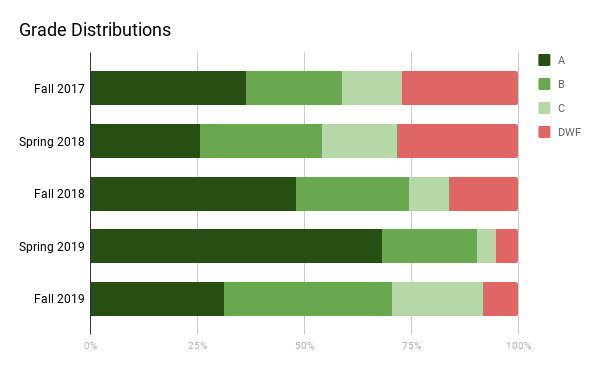
\includegraphics[scale=0.5]{grades.png}
%  \end{center}
%  \end{frame}
  
  \begin{frame}\frametitle{Overview of Team-Based Learning}
  \begin{itemize}
  \item This course uses Team-Based Learning to promote collaboration and allow students to deeply engage with mathematics.
  \item The course is divided into 5 ``modules''.
  \item The first day of each module is the Readiness Assurance Process.
  \item Remaining days are spent working on activities in your teams.
  \end{itemize}
  \end{frame}

  \begin{frame}\frametitle{Readiness Assurance Process}
  \begin{itemize}
  \item In Canvas, you will find a list of the skills you should have {\bf before each module starts}, along with resources to help you prepare.
  \begin{itemize}
  \item Sometimes these skills are from previous courses.
  \item Sometimes these skills are standards from earlier in this course.
    \item Sometimes (but rarely) these are new skills you will learn by watching the videos and answering embedded questions.
  \end{itemize}
  \pause \item On the first day of the module, the Readiness Assurance Checks will ensure you have these skills.
  \begin{itemize}
  \item First, you will individually work some problems
  \item After everyone is done, you will work the same problems again collaboratively as a team.
  \end{itemize}
  \item {\bf The first Readiness Assurance day is Thursday!}
  \end{itemize}
  \end{frame}
  
  
\begin{frame}\frametitle{Class Activities}
Most days we will spend our time working in teams through a series of activities in our teams
\begin{itemize}
\item These activities are designed to help you \textbf{explore} the material.
\item Often, you will not immediately know how to complete them.  You will have all the tools you will need, but will have to apply them in a new way.
\item Sometimes, it will be hard.  That's okay!
\item Research shows these kind of activities lead to deeper learning.
\end{itemize}

\end{frame}

\begin{frame}\frametitle{Teams}
\begin{itemize}
\item I have organized you into teams.
\item I did this pseudo-randomly, ensuring a mix of majors on each team.
\end{itemize}
\end{frame}



\begin{frame}\frametitle{Team Names}
\begin{itemize}
\item Introduce yourselves to each other
\item Decide on a name for your team
\end{itemize}
\end{frame}

%\begin{frame}\frametitle{Team Assets}
%Think about what makes a good team member.  For each member of your team:
%
%\begin{itemize}
%\item List three assets (strengths) that each person brings to the team.
%\pause \item List one thing each member of the team would like to improve at.
%\item Make a list on your team's Jamboard slide.
%\end{itemize}
%\end{frame}


\begin{frame}\frametitle{Team and Class Norms}

In your teams, come up with a list of norms you would like your team (and the class to follow)
\vfill
What things do you want your teammates to do this semester, and what should they expect of you?
\end{frame}

\begin{frame}\frametitle{Class Communication Plan}

How do we want to communicate with each other outside of class?
\vfill
Some options used in the past:
\begin{itemize}
\item Canvas 
\item Discord
\item Slack
\item GroupMe
\end{itemize}

\end{frame}


\begin{frame}\frametitle{Participation Norms}

In your teams, come up with a list of ways you can participate and contribute in class.
\vfill
\begin{itemize}
\item How might you participate during class?
\item How might you participate if you can't come to class? 
\item How might you contribute between class meetings?
\end{itemize}
\end{frame}

\section{Standards Based Grading (SBG)}
%\begin{frame}\frametitle{What does a grade represent?}
%
%In your teams, make a list of all the things a grade in a course represents.
%\vfill
%
%\pause
%What should a grade represent?
%\vfill
%\end{frame}



\begin{frame}\frametitle{Standards Based Grading (SBG)}
Your main job in this course is to \textbf{learn the covered material}
and \textbf{demonstrate that learning to me}.

\vspace{0.2in}
\pause

You will be given several opportunities to demonstrate your learning throughout
the semester, and if
at first you don't succeed, you can try again without any penalty.
\end{frame}

\begin{frame}\frametitle{SBG is different!}
SBG has many advantages
\begin{itemize}
\item You can learn and demonstrate learning at \textbf{your} pace, not the instructor's.
\item No high stakes exams -- you can always reassess at a later date.
\item You can demonstrate mastery in multiple ways.
\end{itemize}
\vfill
But it's different!
\begin{itemize}
\item Some students take some time to adjust.  Unlike many courses you have taken before, \textbf{you will not succeed by only accumulating partial understanding.}
\item The best advice former students give is to not delay in demonstrating your learning
\end{itemize}
\end{frame}




\begin{frame}\frametitle{SBG}
The course material is broken down into 24 learning \textbf{standards}.
\begin{itemize}
\item Each attempted exercise will be simply marked according to whether or not
      your solution \textbf{demonstrates excellence} of the relevant standards.
\item Your grade is calculated based on how many standards you demonstrate excellence of \textbf{twice}.
\item Standards will be assessed several times, and there's no penalty for
      incorrect solutions. So, if you don't succeed the first time,
      keep practicing and try again!
\end{itemize}
\end{frame}

\begin{frame}\frametitle{Assessment Opportunities}
Checkmarks may be earned as follows.
\begin{itemize}
\item {\bf Quizzes}: Most weeks, we will have a quiz (usually on TBD). 
\item {\bf Exams}: Periodically we will have longer assessments (usually on TBD).
\item {\bf On Demand Reassessments}: You can also complete a reassessment of an individual standard whenever you like.
\end{itemize}

\pause

\vspace{0.2in}

The assessment method (quiz/exam/etc.) you used to earn a checkmark
isn't important: \textbf{I only care that you
learn the material and demonstrate that learning to me before the end of the
semester!}
\end{frame}

\begin{frame}\frametitle{A tale of two students}
These two students took very different paths, but both earned the same grade.
\begin{center}
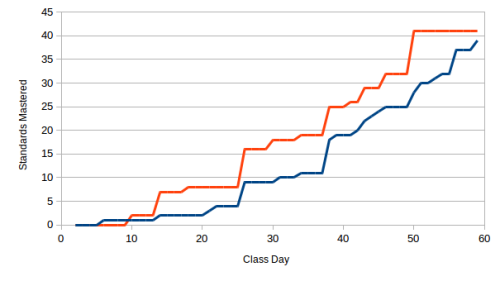
\includegraphics[scale=0.7]{student-comparison.png}
\end{center}
\end{frame}



\begin{frame}\frametitle{Interpreting Feedback}
On each assessment, for each standard you will receive one of the following marks.
\begin{itemize}
\item {\bf Demonstrated Excellence}: Great job!  Check off another box on your progress sheet.
\item {\bf Minor Revision Needed} means you have a minor mistake, unrelated to the standard. Often these are arithmetic mistakes or notation errors. You can rework the same problem, fixing your mistakes, and resubmit to demonstrate mastery.
\item {\bf Reassessment Needed} means you made a good faith effort and demonstrated
      partial understanding, but not complete mastery. You will need to \textbf{reassess} on the next quiz, exam, and/or in an on demand reassessment.
\end{itemize}

\vspace{0.2in}

\end{frame}




\begin{frame}\frametitle{Course Grades}

\begin{center}
\begin{tabular}{ll} \hline
A & Demonstrate excellence twice on 22 standards\\ \hline
B & Demonstrate excellence twice on 20 standards\\ \hline
C & Demonstrate excellence twice on 17 standards\\ \hline
D & Demonstrate excellence twice on 15 standards\\ \hline
\end{tabular}
\end{center}

\end{frame}


\begin{frame}\frametitle{Other Assessments}
In addition to mastering content, I will ask you to do some other things because experience shows these help students learn.
\begin{itemize}
%\item Class Attendance
\item Individual \& Team Readiness Assurance Checks
\item Reflections 
\item Homework
\item Final
\end{itemize}
\end{frame}

\section{Logistics}

\begin{frame}\frametitle{Student Hours (Office Hours)}
Student Hours are meant to be for the following things (among others):
\begin{enumerate}
\item Questions
\item Conversations
\item Feedback
\end{enumerate}

\vspace{0.2in}

Student Hours are TR 9-9:30, 10:45-11, 12:15-1 and Wednesday 12-3. My office is 306 MSPB.
\end{frame}



\begin{frame}\frametitle{Homework}
Homework is practice.  A link to homework exercises, organized by standard, is available in Canvas.
\begin{itemize}
\item I will not collect or grade homework.
\item You will need to submit 3 homework problems in order to complete an on-demand reassessment
\item If you need help or feedback, come to my student hours 
\end{itemize}
\end{frame}



\begin{frame}\frametitle{Rescheduling Due Dates}

Use the form in Canvas whenever you need to reschedule a due date.

\end{frame}



\begin{frame}\frametitle{Canvas}
\begin{center}
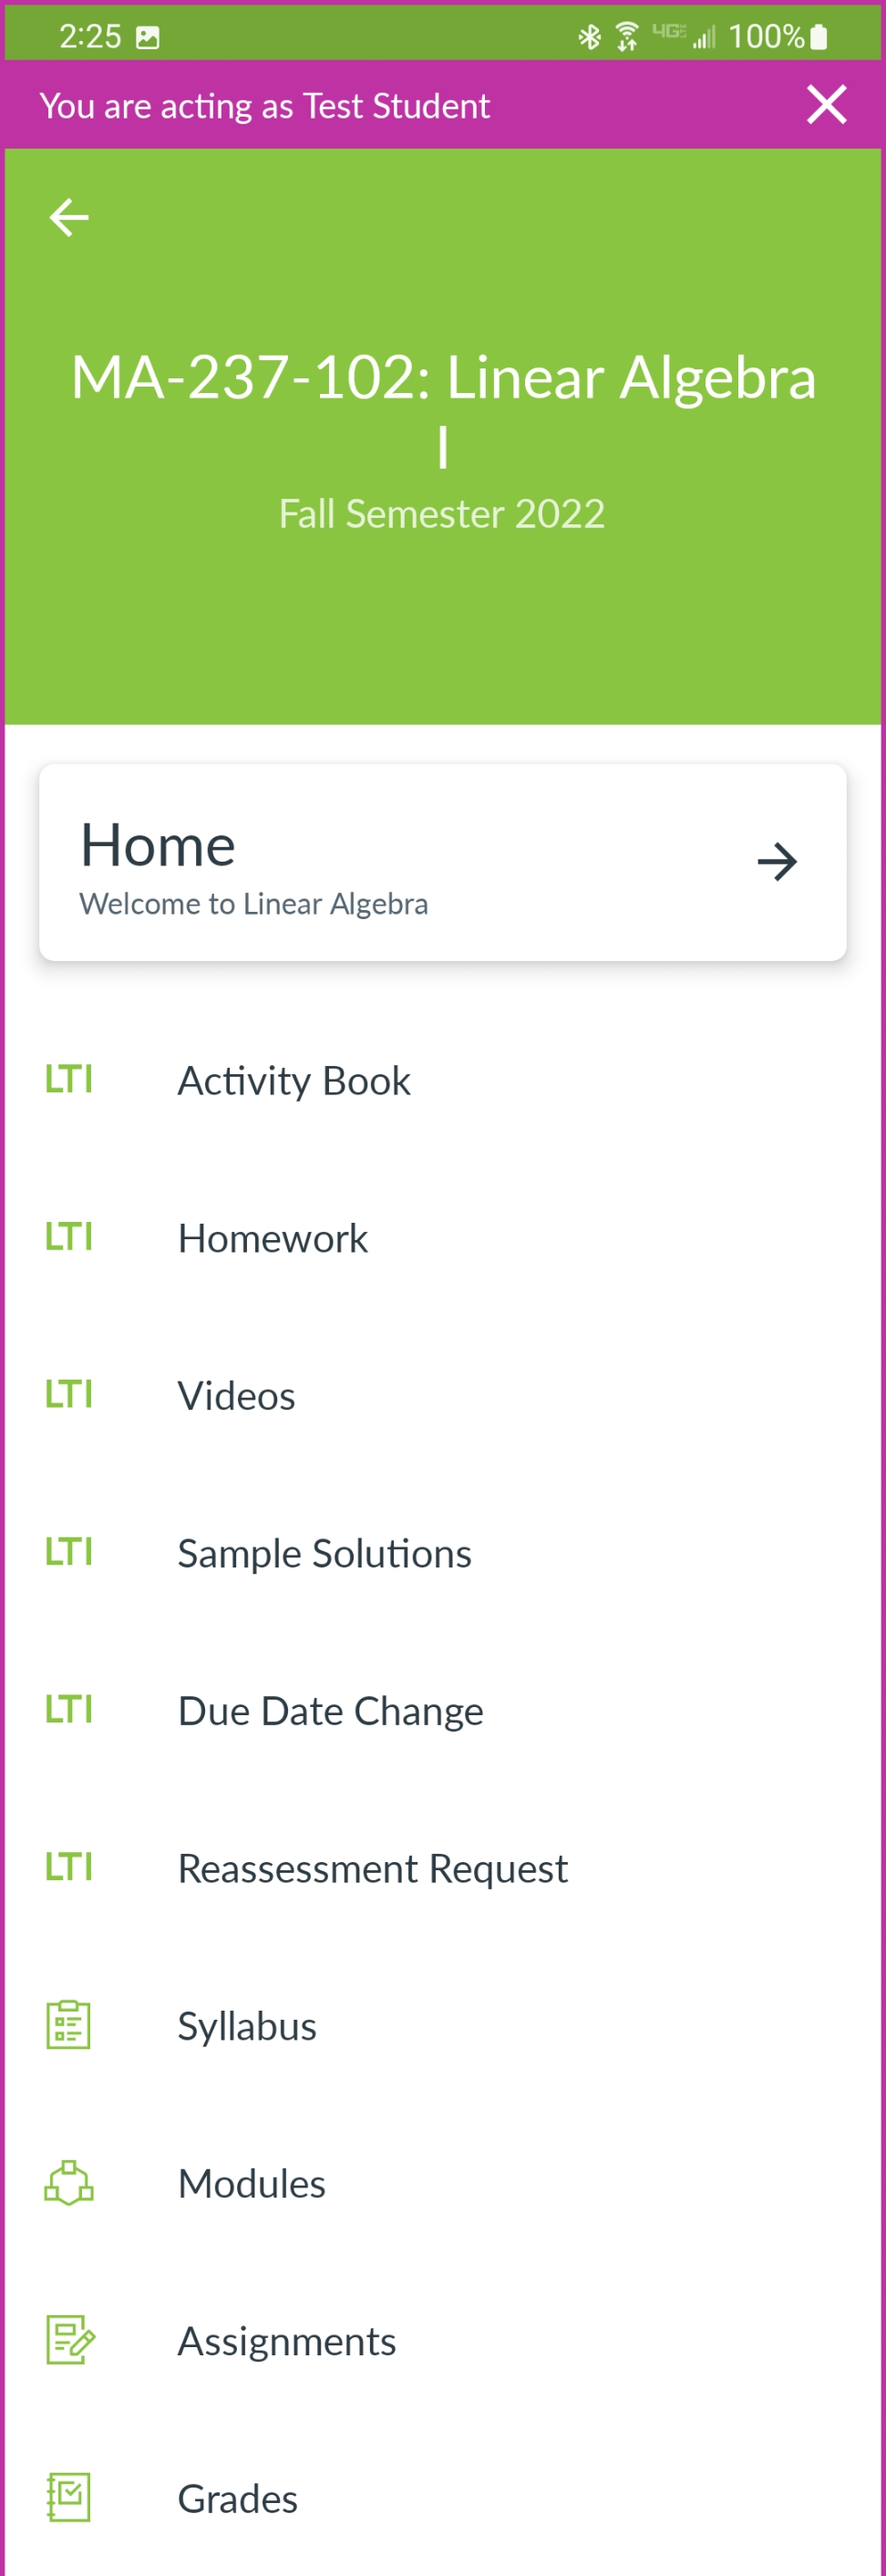
\includegraphics[height=0.9\textheight]{canvas_menu.jpg}
\end{center}
\end{frame}

\begin{frame}\frametitle{Canvas}
\begin{center}
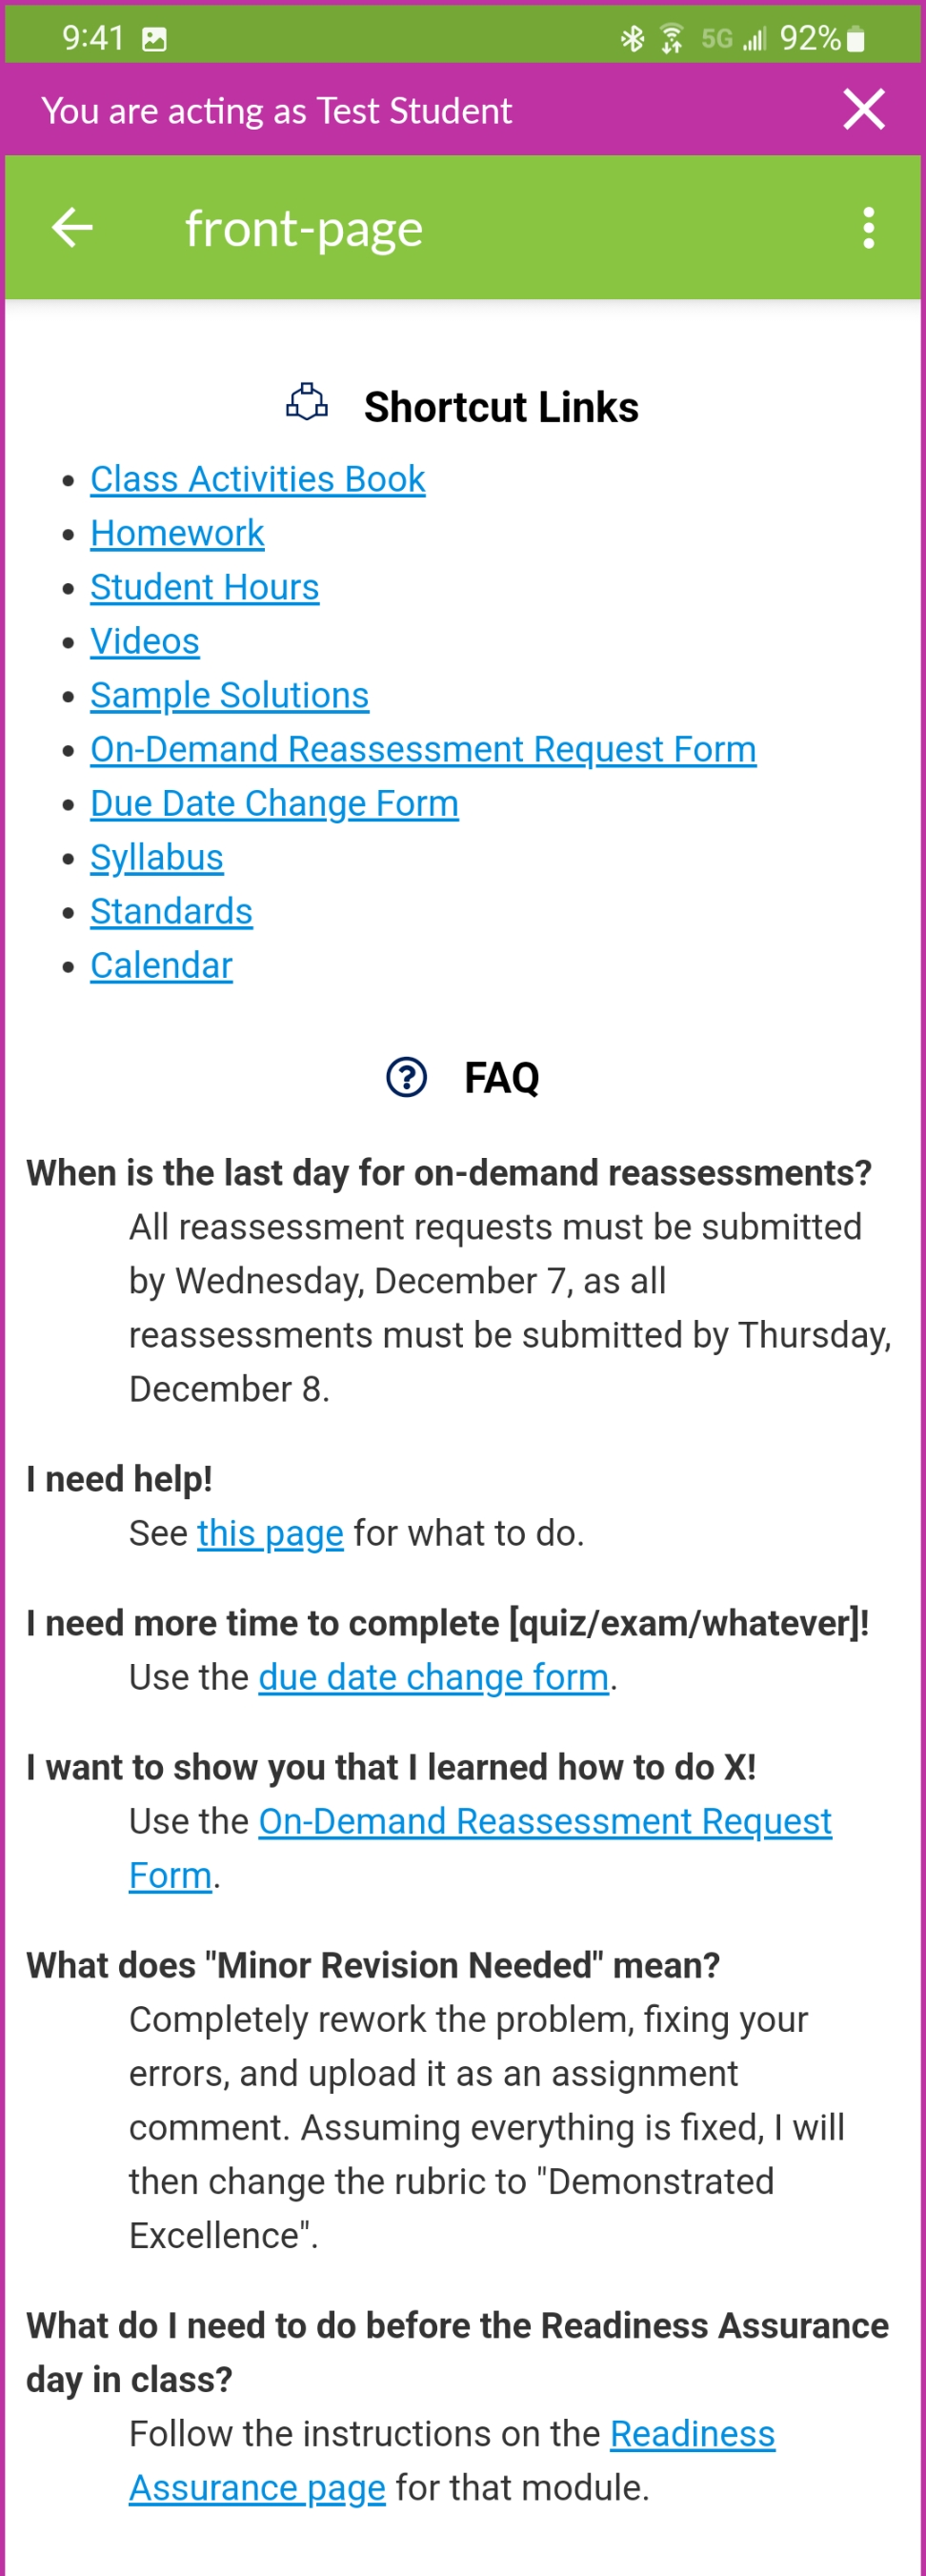
\includegraphics[height=0.9\textheight]{canvas_more.jpg}
\end{center}
\end{frame}

\begin{frame}\frametitle{Two things to decide}
\begin{itemize}
\item Do we want to spend class time on assessments?
\pause \item What day do we want to do assessments?
\end{itemize}
\end{frame}

\begin{frame}\frametitle{Questions}

\begin{itemize}
\item Do you have office hours?
\item Do I need the textbook?
\item How does linear algebra have real world applications?
\item How will class operate?
\item What is the difference between linear algebra and algebra?
\end{itemize}
\end{frame}



\begin{frame}\frametitle{Reminder}
The first Readiness Assurance Day is Thursday!
\end{frame}



\end{document}
